\documentclass{llncs}
%%%%%%%%%%%%%%%%%%%%%%%%%%%%%%%%%%%%%%%%%%%%%%%%%%%%%%%%%%%
%% package sillabazione italiana e uso lettere accentate
\usepackage[latin1]{inputenc}
\usepackage[english]{babel}
\usepackage[T1]{fontenc}
%%%%%%%%%%%%%%%%%%%%%%%%%%%%%%%%%%%%%%%%%%%%%%%%%%%%%%%%%%%%%

\usepackage{url}
\usepackage{xspace}
\usepackage{hyperref}
\usepackage{listings}

\makeatletter
%%%%%%%%%%%%%%%%%%%%%%%%%%%%%% User specified LaTeX commands.
\usepackage{manifest}

\makeatother

%%%%%%%
 \newif\ifispdf
 \ifx\pdfoutput\undefined
 \ispdffalse % we are not running PDFLaTeX
 \else
 \pdfoutput=1 % we are running PDFLaTeX
 \ispdftrue
 \fi
%%%%%%%
 \ifispdf
 \usepackage[pdftex]{graphicx}
 \else
 \usepackage{graphicx}
 \fi
%%%%%%%%%%%%%%%
 \ifispdf
 \DeclareGraphicsExtensions{.pdf, .jpg, .tif,.png}
 \else
 \DeclareGraphicsExtensions{.eps, .jpg}
 \fi
%%%%%%%%%%%%%%%

\newcommand{\action}[1]{\texttt{#1}\xspace}
\newcommand{\code}[1]{{\small{\texttt{#1}}}\xspace}
\newcommand{\codescript}[1]{{\scriptsize{\texttt{#1}}}\xspace}

% Cross-referencing
\newcommand{\labelsec}[1]{\label{sec:#1}}
\newcommand{\xs}[1]{\sectionname~\ref{sec:#1}}
\newcommand{\xsp}[1]{\sectionname~\ref{sec:#1} \onpagename~\pageref{sec:#1}}
\newcommand{\labelssec}[1]{\label{ssec:#1}}
\newcommand{\xss}[1]{\subsectionname~\ref{ssec:#1}}
\newcommand{\xssp}[1]{\subsectionname~\ref{ssec:#1} \onpagename~\pageref{ssec:#1}}
\newcommand{\labelsssec}[1]{\label{sssec:#1}}
\newcommand{\xsss}[1]{\subsectionname~\ref{sssec:#1}}
\newcommand{\xsssp}[1]{\subsectionname~\ref{sssec:#1} \onpagename~\pageref{sssec:#1}}
\newcommand{\labelfig}[1]{\label{fig:#1}}
\newcommand{\xf}[1]{\figurename~\ref{fig:#1}}
\newcommand{\xfp}[1]{\figurename~\ref{fig:#1} \onpagename~\pageref{fig:#1}}
\newcommand{\labeltab}[1]{\label{tab:#1}}
\newcommand{\xt}[1]{\tablename~\ref{tab:#1}}
\newcommand{\xtp}[1]{\tablename~\ref{tab:#1} \onpagename~\pageref{tab:#1}}

% Category Names
\newcommand{\sectionname}{Section}
\newcommand{\subsectionname}{Subsection}
\newcommand{\sectionsname}{Sections}
\newcommand{\subsectionsname}{Subsections}
\newcommand{\secname}{\sectionname}
\newcommand{\ssecname}{\subsectionname}
\newcommand{\secsname}{\sectionsname}
\newcommand{\ssecsname}{\subsectionsname}
\newcommand{\onpagename}{on page}

\newcommand{\xauthA}{Luca Mella}
\newcommand{\xauthB}{NameB StudentB}
\newcommand{\xauthC}{NameC StudentC}
\newcommand{\xfaculty}{II Faculty of Engineering}
\newcommand{\xunibo}{Alma Mater Studiorum -- University of Bologna}
\newcommand{\xaddrBO}{viale Risorgimento 2}
\newcommand{\xaddrCE}{via Venezia 52}
\newcommand{\xcityBO}{40136 Bologna, Italy}
\newcommand{\xcityCE}{47521 Cesena, Italy}


\begin{document}

\title{Laboratory Report\\Progetto Reti 2013}

\author{\xauthA}

\institute{
\xunibo\\\xaddrCE, \xcityCE\\\email\ luca.mella@studio.unibo.it
}

\maketitle

\lstset{frame=lrb,xleftmargin=\fboxsep , xrightmargin=-\fboxsep}

%===========================================================================
\section{OSPF Single Area}
\labelsec{OSPF_single_area}

The first laboratory experience consisted in setting-up the network shown in figure \ref{fig:ospf_topology}. In our specific case $X=15$ and $Y=16$. We configured the OSPF routing protocol in all the routers present in the topology diagram. 

\begin{figure}
\centering
\includegraphics[width=1.0\textwidth]{../e1/topologia.png}
\caption{Laboratory tolopogy}
\label{fig:ospf_topology}
\end{figure}

The main goal of the simulation was to observe how OSPF network react to network changes, so , for the sake of simplicity, we configured all these router in the same routing area (\emph{backbone area}).\\
\newpage
\lstset{language=sh, caption=Router Cisco 2801A OSPF configuration,  basicstyle=\ttfamily\scriptsize , breaklines=true}
\begin{lstlisting}
2801A#show running config
router ospf 15
 router-id 172.30.15.2
 log-adjacency-changes
 network 10.15.16.0 0.0.0.3 area 0
 network 172.16.15.4 0.0.0.3 area 0
 network 172.30.15.2 0.0.0.0 area 0
 
2801A#show ip ospf neighbor 
Neighbor ID     Pri   State      Dead Time   Address      Interface
172.30.16.2       0   FULL/  -   00:00:37    10.15.16.2   FastEth0/3/0.1516
172.30.15.1       1   FULL/BDR   00:00:38    172.16.15.5  FastEth0/1.15
\end{lstlisting}
\lstset{language=sh, caption=Router Cisco 2801B OSPF configuration,  basicstyle=\ttfamily\scriptsize , breaklines=true}
\begin{lstlisting}
2801B#show running config
router ospf 16
 router-id 172.30.16.2
 log-adjacency-changes
 network 10.15.16.0 0.0.0.3 area 0
 network 172.16.16.4 0.0.0.3 area 0
 network 172.30.16.2 0.0.0.0 area 0
 
2801B#show ip ospf neighbor 
Neighbor ID     Pri   State      Dead Time   Address      Interface
172.30.15.2       0   FULL/  -   00:00:32    10.15.16.1   Vlan1
172.30.16.1       1   FULL/BDR   00:00:36    172.16.16.5  FastEth0/1.16
\end{lstlisting}

Digging the network database make possible to obtain additional information about links, their status and their type. In the following listing part of the routing databases are reported.
\\
\lstset{language=sh, caption=Router Cisco 2801A network database,  basicstyle=\ttfamily\scriptsize , breaklines=true}
\begin{lstlisting}
2801A#show ip ospf database network 

            OSPF Router with ID (172.30.15.2) (Process ID 15)

		Net Link States (Area 0)

  LS Type: Network Links
  Link State ID: 172.16.15.1 (address of Designated Router)
  Network Mask: /30
	Attached Router: 172.30.15.3
	Attached Router: 172.30.15.1
  LS Type: Network Links
  Link State ID: 172.16.15.6 (address of Designated Router)
  Network Mask: /30
        Attached Router: 172.30.15.2
        Attached Router: 172.30.15.1
  LS Type: Network Links
  Link State ID: 172.16.16.2 (address of Designated Router)
  Network Mask: /30
        Attached Router: 172.30.15.3
        Attached Router: 172.30.16.1
  LS Type: Network Links
  Link State ID: 172.16.16.6 (address of Designated Router)
  Network Mask: /30
        Attached Router: 172.30.16.2
        Attached Router: 172.30.16.1
\end{lstlisting}
\lstset{language=sh, caption=Router Cisco 2801A database router,  basicstyle=\ttfamily\scriptsize , breaklines=true}
\begin{lstlisting}
2801A#show ip ospf database router 

            OSPF Router with ID (172.30.15.2) (Process ID 15)

		Router Link States (Area 0)
		
  LS Type: Router Links
  Link State ID: 172.30.15.1
    Link connected to: a Stub Network
     (Link ID) Network/subnet number: 192.168.115.0
     (Link Data) Network Mask: 255.255.255.0
    Link connected to: a Transit Network
     (Link ID) Designated Router address: 172.16.15.1
     (Link Data) Router Interface address: 172.16.15.2
    Link connected to: a Transit Network
     (Link ID) Designated Router address: 172.16.15.6
     (Link Data) Router Interface address: 172.16.15.5
    Link connected to: a Stub Network
     (Link ID) Network/subnet number: 172.30.15.1
     (Link Data) Network Mask: 255.255.255.255
  LS Type: Router Links
  Link State ID: 172.30.15.2
    Link connected to: a Stub Network
     (Link ID) Network/subnet number: 172.30.15.2
     (Link Data) Network Mask: 255.255.255.255
    Link connected to: another Router (point-to-point)
     (Link ID) Neighboring Router ID: 172.30.16.2
     (Link Data) Router Interface address: 10.15.16.1
    Link connected to: a Stub Network
     (Link ID) Network/subnet number: 10.15.16.0
     (Link Data) Network Mask: 255.255.255.252
    Link connected to: a Transit Network
     (Link ID) Designated Router address: 172.16.15.6
     (Link Data) Router Interface address: 172.16.15.6  
  LS Type: Router Links
  Link State ID: 172.30.15.3
    Link connected to: a Transit Network
     (Link ID) Designated Router address: 172.16.15.1
     (Link Data) Router Interface address: 172.16.15.1
    Link connected to: a Transit Network
     (Link ID) Designated Router address: 172.16.16.2
     (Link Data) Router Interface address: 172.16.16.1
  LS Type: Router Links
  Link State ID: 172.30.16.1
    Link connected to: a Stub Network
     (Link ID) Network/subnet number: 192.168.116.0
     (Link Data) Network Mask: 255.255.255.0   
    Link connected to: a Transit Network
     (Link ID) Designated Router address: 172.16.16.2
     (Link Data) Router Interface address: 172.16.16.2
    Link connected to: a Transit Network
     (Link ID) Designated Router address: 172.16.16.6
     (Link Data) Router Interface address: 172.16.16.5
    Link connected to: a Stub Network
     (Link ID) Network/subnet number: 172.30.16.1 # <== router id netlabY
     (Link Data) Network Mask: 255.255.255.255
       TOS 0 Metrics: 10   # <== other ones (not reported) are 1
  LS Type: Router Links
  Link State ID: 172.30.16.2
    Link connected to: a Stub Network
     (Link ID) Network/subnet number: 172.30.16.2
     (Link Data) Network Mask: 255.255.255.255
    Link connected to: another Router (point-to-point)
     (Link ID) Neighboring Router ID: 172.30.15.2
     (Link Data) Router Interface address: 10.15.16.2
    Link connected to: a Stub Network
     (Link ID) Network/subnet number: 10.15.16.0
     (Link Data) Network Mask: 255.255.255.252
    Link connected to: a Transit Network
     (Link ID) Designated Router address: 172.16.16.6
     (Link Data) Router Interface address: 172.16.16.6
\end{lstlisting}
And also we report the resulting routing table of the Cisco routers.
\lstset{language=sh, caption=Router Cisco 2801A and 2801B resulting routing,  basicstyle=\ttfamily\scriptsize , breaklines=true}
\begin{lstlisting}

ROUTING TABLE CISCO 2801A

C  192.168.8.0/24 is directly connected, FastEthernet0/0
   172.16.0.0/30 is subnetted, 4 subnets
O     172.16.16.4 [110/2] via 10.15.16.2, 00:24:31, FastEthernet0/3/0.1516
O     172.16.16.0 [110/3] via 172.16.15.5, 00:03:29, FastEthernet0/1.15
                  [110/3] via 10.15.16.2, 00:03:39, FastEthernet0/3/0.1516
O     172.16.15.0 [110/2] via 172.16.15.5, 00:05:04, FastEthernet0/1.15
C     172.16.15.4 is directly connected, FastEthernet0/1.15
   172.30.0.0/32 is subnetted, 4 subnets
O     172.30.16.2 [110/2] via 10.15.16.2, 00:24:31, FastEthernet0/3/0.1516
O     172.30.16.1 [110/12] via 10.15.16.2, 00:16:49, FastEthernet0/3/0.1516
O     172.30.15.1 [110/11] via 172.16.15.5, 00:14:34, FastEthernet0/1.15
C     172.30.15.2 is directly connected, Loopback15
O  192.168.115.0/24 [110/2] via 172.16.15.5, 00:05:40, FastEthernet0/1.15
   10.0.0.0/30 is subnetted, 1 subnets
C     10.15.16.0 is directly connected, FastEthernet0/3/0.1516
O  192.168.116.0/24 [110/3] via 10.15.16.2, 00:06:40, FastEthernet0/3/0.1516

ROUTING TABLE CISCO 2801B

C  192.168.8.0/24 is directly connected, FastEthernet0/0
   172.16.0.0/30 is subnetted, 4 subnets
C     172.16.16.4 is directly connected, FastEthernet0/1.16
O     172.16.16.0 [110/2] via 172.16.16.5, 00:02:37, FastEthernet0/1.16
O     172.16.15.0 [110/3] via 172.16.16.5, 00:02:27, FastEthernet0/1.16
                  [110/3] via 10.15.16.1, 00:04:01, Vlan1
O     172.16.15.4 [110/2] via 10.15.16.1, 00:23:38, Vlan1
   172.30.0.0/32 is subnetted, 4 subnets
C     172.30.16.2 is directly connected, Loopback16
O     172.30.16.1 [110/11] via 172.16.16.5, 00:15:46, FastEthernet0/1.16
O     172.30.15.1 [110/12] via 10.15.16.1, 00:13:31, Vlan1
O     172.30.15.2 [110/2] via 10.15.16.1, 00:23:38, Vlan1
O  192.168.115.0/24 [110/3] via 10.15.16.1, 00:04:38, Vlan1
   10.0.0.0/30 is subnetted, 1 subnets
C     10.15.16.0 is directly connected, Vlan1
O  192.168.116.0/24 [110/2] via 172.16.16.5, 00:05:37, FastEthernet0/1.16
\end{lstlisting}


\lstset{language=sh, caption=Traceroute from netlab15 host to netlab16 host,  basicstyle=\ttfamily\scriptsize , breaklines=true}
\begin{lstlisting}
traceroute -n 192.168.116.1
traceroute to 192.168.116.1 (192.168.116.1), 30 hops max, 60 byte packets
 1  192.168.115.2  0.191 ms  0.177 ms  0.156 ms
 2  172.16.15.1  5.923 ms  6.056 ms  6.185 ms
 3  172.16.16.2  5.543 ms  5.677 ms *
 4  192.168.116.1  4.657 ms  4.667 ms  4.700 ms
\end{lstlisting}

\subsubsection{Link Failure}

After a failure in one of the link network state should be updated after a \emph{RouterDeadInterval} time, this mean that in case of failure we should assist to another LSA Update propagation through the interested routers.\\
So we disconnect an interface of the \emph{Huawei} router - see fig.\ref{fig:ospf_topology} - and we observed the transit of new LSA Update packets
\begin{figure}
\centering
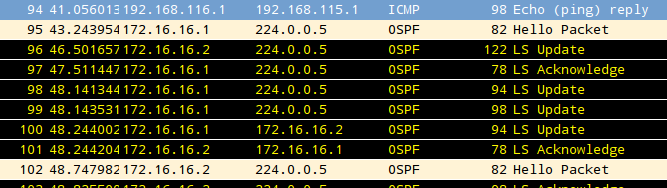
\includegraphics[width=1.0\textwidth]{../e1/caduta_connessione_lsaupdate.png}
\caption{LSA Update due to link failure}
\label{fig:caduta_connessione_lsaupdate}
\end{figure}

As the reader can see in fig.\ref{fig:lsa update after failure}, new LSA Update contains only 3 link specification while previously there were 4.\\
After receiving this update, other routers will recompute paths and modify their routing table.

\begin{figure}
\centering
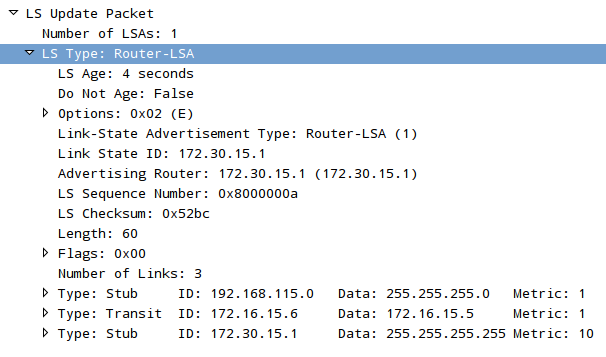
\includegraphics[width=1.0\textwidth]{../e1/lsa_update_after_failure.png}
\caption{LSA Update details}
\label{fig:lsa update after failure}
\end{figure}

%\lstset{language=sh, caption=Old LSA Update,  basicstyle=\ttfamily\scriptsize , breaklines=true}
%\begin{lstlisting}
%  LS Type: Router Links
%  Link State ID: 172.30.15.1
%    Link connected to: a Stub Network
%     (Link ID) Network/subnet number: 192.168.115.0
%     (Link Data) Network Mask: 255.255.255.0
%    Link connected to: a Transit Network
%     (Link ID) Designated Router address: 172.16.15.1
%     (Link Data) Router Interface address: 172.16.15.2
%    Link connected to: a Transit Network
%     (Link ID) Designated Router address: 172.16.15.6
%     (Link Data) Router Interface address: 172.16.15.5
%    Link connected to: a Stub Network
%     (Link ID) Network/subnet number: 172.30.15.1
%     (Link Data) Network Mask: 255.255.255.255
%\end{lstlisting}

%===========================================================================
\newpage
\section{OSPF Multi Area}
\labelsec{OSPF_multi_area}
In the second laboratory experience we reconfigured the network shown in figure \ref{fig:ospf_topology} by subdividing the macro routing area 0 into smaller routing areas. As always $X=15$ and $Y=16$. The resulting topology is shown in fig.\ref{fig:ospf2_topology}.

\begin{figure}
\centering
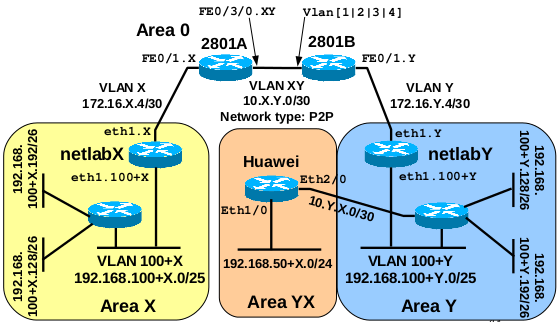
\includegraphics[width=1.0\textwidth]{../e2/topology.png}
\caption{Laboratory tolopogy with multiple routing areas}
\label{fig:ospf2_topology}
\end{figure}

In this laboratory session the main goal was to use \emph{aggregation} for ease OSPF database and then configure a \emph{virtual link} in order to make area 1615 reachable even from area 15.\\
In the following code listing we report the routing table of netlab15 router (area 15) before any aggregation, in fact area 16 compare in routing table with all its subnets. 
\\
\lstset{language=sh, caption=Routing table of router 192.168.115.1 ,  basicstyle=\ttfamily\scriptsize , breaklines=true}
\begin{lstlisting}
netlab15-ospfd# show ip ospf route    
============ OSPF network routing table ============
N IA 10.15.16.0/30         [12] area: 0.0.0.15
                           via 192.168.115.2, eth1.115
N IA 172.16.15.4/30        [11] area: 0.0.0.15
                           via 192.168.115.2, eth1.115
N IA 172.16.16.4/30        [13] area: 0.0.0.15
                           via 192.168.115.2, eth1.115
N IA 172.30.15.1/32        [20] area: 0.0.0.15
                           via 192.168.115.2, eth1.115
N IA 172.30.15.2/32        [12] area: 0.0.0.15
                           via 192.168.115.2, eth1.115
N IA 172.30.16.1/32        [23] area: 0.0.0.15
                           via 192.168.115.2, eth1.115
N IA 172.30.16.2/32        [13] area: 0.0.0.15				
                           via 192.168.115.2, eth1.115
N    172.30.115.1/32       [10] area: 0.0.0.15
                           directly attached to lo
N IA 172.30.116.1/32       [24] area: 0.0.0.15				
                           via 192.168.115.2, eth1.115
N    192.168.115.0/25      [10] area: 0.0.0.15
                           directly attached to eth1.115
N    192.168.115.128/26    [10] area: 0.0.0.15
                           directly attached to eth1.1152
N    192.168.115.192/26    [10] area: 0.0.0.15
                           directly attached to eth1.1151
N IA 192.168.116.0/25      [14] area: 0.0.0.15				<====
                           via 192.168.115.2, eth1.115
N IA 192.168.116.128/26    [24] area: 0.0.0.15				<====
                           via 192.168.115.2, eth1.115
N IA 192.168.116.192/26    [24] area: 0.0.0.15				<====
                           via 192.168.115.2, eth1.115
\end{lstlisting}

After aggregation the aggregation, the internal router 192.168.115.1 (area 15), present a more compact routing table, in fact area 16 sub-networks have been summarized in a single /24.\\
However area 1615 is still unreachable because no one of their LSA Update reach area 15.
\\
\lstset{language=sh, caption=Routing table of router 192.168.115.1 after aggregation basicstyle=\ttfamily\scriptsize , breaklines=true}
\begin{lstlisting}
netlab13-ospfd# show ip ospf route 
============ OSPF network routing table ============
N IA 10.15.16.0/30         [12] area: 0.0.0.15
                           via 192.168.115.2, eth1.115
N IA 10.16.15.0/30         [24] area: 0.0.0.15
                           via 192.168.115.2, eth1.115
N IA 172.16.15.4/30        [11] area: 0.0.0.15
                           via 192.168.115.2, eth1.115
N IA 172.16.16.4/30        [13] area: 0.0.0.15
                           via 192.168.115.2, eth1.115
N IA 172.30.15.1/32        [20] area: 0.0.0.15
                           via 192.168.115.2, eth1.115
N IA 172.30.15.2/32        [12] area: 0.0.0.15
                           via 192.168.115.2, eth1.115
N IA 172.30.16.1/32        [23] area: 0.0.0.15
                           via 192.168.115.2, eth1.115
N IA 172.30.16.2/32        [13] area: 0.0.0.15
                           via 192.168.115.2, eth1.115
N    172.30.115.1/32       [10] area: 0.0.0.15
                           directly attached to lo
N IA 172.30.116.1/32       [24] area: 0.0.0.15
                           via 192.168.115.2, eth1.115
N    192.168.115.0/25      [10] area: 0.0.0.15
                           directly attached to eth1.115
N    192.168.115.128/26    [10] area: 0.0.0.15
                           directly attached to eth1.1152
N    192.168.115.192/26    [10] area: 0.0.0.15
                           directly attached to eth1.1151
N IA 192.168.116.0/24      [24] area: 0.0.0.15			<====
                           via 192.168.115.2, eth1.115
\end{lstlisting}

In order to make area 1615 reachable from other areas is necessary to virtually link it to the backbone area, permitting to its LSA Update to be perceived by other ABR.\\
The OSPF way to achieve this objective is through \emph{virtual link}:
\begin{verbatim}
[Quidway-ospf-area]vlink-peer <router ID>
\end{verbatim}
Before linking area 1615 with backbone could be useful to aggregate area 16 subnets too, this will lower the LSA Update traffic.
\\
\lstset{language=sh, caption=Routing table of router 192.168.115.1 after virtual link, basicstyle=\ttfamily\scriptsize , breaklines=true}
\begin{lstlisting}
netlab13-ospfd# show ip ospf route 
============ OSPF network routing table ============
N IA 10.15.16.0/30         [12] area: 0.0.0.15
                           via 192.168.115.2, eth1.115
N IA 10.16.15.0/30         [24] area: 0.0.0.15
                           via 192.168.115.2, eth1.115
N IA 172.16.15.4/30        [11] area: 0.0.0.15
                           via 192.168.115.2, eth1.115
N IA 172.16.16.4/30        [13] area: 0.0.0.15
                           via 192.168.115.2, eth1.115
N IA 172.30.15.1/32        [20] area: 0.0.0.15
                           via 192.168.115.2, eth1.115
N IA 172.30.15.2/32        [12] area: 0.0.0.15
                           via 192.168.115.2, eth1.115
N IA 172.30.15.3/32        [25] area: 0.0.0.15
                           via 192.168.115.2, eth1.115
N IA 172.30.16.1/32        [23] area: 0.0.0.15
                           via 192.168.115.2, eth1.115
N IA 172.30.16.2/32        [13] area: 0.0.0.15
                           via 192.168.115.2, eth1.115
N    172.30.115.1/32       [10] area: 0.0.0.15
                           directly attached to lo
N IA 172.30.116.1/32       [24] area: 0.0.0.15
                           via 192.168.115.2, eth1.115
N IA 192.168.66.0/24       [25] area: 0.0.0.15		<====
                           via 192.168.115.2, eth1.115
N    192.168.115.0/25      [10] area: 0.0.0.15
                           directly attached to eth1.115
N    192.168.115.128/26    [10] area: 0.0.0.15
                           directly attached to eth1.1152
N    192.168.115.192/26    [10] area: 0.0.0.15
                           directly attached to eth1.1151
N IA 192.168.116.0/24      [24] area: 0.0.0.15
                           via 192.168.115.2, eth1.115
\end{lstlisting}


\lstset{language=sh, caption=OSPF database of backbone router Cisco 2801A, basicstyle=\ttfamily\scriptsize , breaklines=true}
\begin{lstlisting}
2801A#show ip ospf database 

            OSPF Router with ID (172.30.15.2) (Process ID 15)

		Router Link States (Area 0)
Link ID         ADV Router      
172.30.15.1     172.30.15.1     
172.30.15.2     172.30.15.2     
172.30.15.3     172.30.15.3     
172.30.16.1     172.30.16.1   
172.30.16.2     172.30.16.2    
		Net Link States (Area 0)
Link ID         ADV Router    
172.16.15.6     172.30.15.2   
172.16.16.6     172.30.16.2   
		Summary Net Link States (Area 0)
Link ID         ADV Router     
10.16.15.0      172.30.15.3
10.16.15.0      172.30.16.1
172.30.15.3     172.30.15.3
172.30.15.3     172.30.16.1
172.30.115.1    172.30.15.1
172.30.116.1    172.30.15.3
172.30.116.1    172.30.16.1
192.168.66.0    172.30.15.3
192.168.115.0   172.30.15.1
192.168.116.0   172.30.15.3
192.168.116.0   172.30.16.1
\end{lstlisting}

%===========================================================================
\section{MPLS Basic Configuration}
\labelsec{MPLS_basic}

In this laboratory experience we set-up a basic MPLS as shown in \ref{fig:mpls1_topology}, as always $X=15$ and $Y=16$. 

\begin{figure}
\centering
\includegraphics[width=1.0\textwidth]{../e3/topologia.png}
\caption{Laboratory tolopogy with multiple routing areas}
\label{fig:mpls1_topology}
\end{figure}

This laboratory session was preparatory for the following ones, that will face Virtual Private LAN and traffic engineering. So the main goal of this experience was to prepare the test bed for the following laboratory sessions and practice with MPLS configuration.\\
In order to make this lab session more educational we specified different tag values for better observing MPLS label switching.\\
In this scenario Cisco 2801A and Cisco 2801B are Label Edge Router (LER), while Cisco 1841C is a Label Swithed Rouer (LSR)\footnote{Actually all MPLS router are LSR.}\\

\lstset{language=sh, caption=MPLS Neighborhood on router Cisco 1841C, basicstyle=\ttfamily\scriptsize , breaklines=true}
\begin{lstlisting}
1841C#show mpls ldp  neighbor 
							<==== Cisco 2801A
    Peer LDP Ident: 172.30.15.2:0; Local LDP Ident 10.10.100.200:0 
	TCP connection: 172.30.15.2.55404 - 10.10.100.200.646
	State: Oper; Msgs sent/rcvd: 17/18; Downstream
	Up time: 00:02:10
	LDP discovery sources:
	  FastEthernet0/1, Src IP addr: 10.10.100.2
        Addresses bound to peer LDP Ident:
          192.168.8.249   172.16.15.6     10.10.100.2     10.15.16.1      
          172.30.15.2 
							<==== Cisco 2801B
    Peer LDP Ident: 172.30.16.2:0; Local LDP Ident 10.10.100.200:0 
	TCP connection: 172.30.16.2.11259 - 10.10.100.200.646
	State: Oper; Msgs sent/rcvd: 15/15; Downstream
	Up time: 00:00:55
	LDP discovery sources:
	  Vlan1, Src IP addr: 10.10.200.2
        Addresses bound to peer LDP Ident:
          192.168.8.250   172.16.16.6     172.30.16.2     10.10.200.2     
\end{lstlisting}

\lstset{language=sh, caption=MPLS Label configuration in all LSR, basicstyle=\ttfamily\scriptsize , breaklines=true}
\begin{lstlisting}
2801A#show mpls label range 
Downstream Generic label region: Min/Max label: 1000/1999

2801B#show mpls label range 
Downstream Generic label region: Min/Max label: 2000/2999

1841C#show mpls label range 
Downstream Generic label region: Min/Max label: 3000/3999
\end{lstlisting}

From MPLS forwarding table is possible to reconstruct an hypothetical label switching dynamic of a packet coming from 192.168.115.0/24 to 192.168.116.0/24:
\begin{itemize}
\item It will be marked with label 1006 from 2801A.
\item Once tagged it will be forwarded as specified in forwarding table: label will be changed from 1006 to 3007.
\item Then 1841C change again label from 3007 to 2001 and then forward it in Vl1 interface.
\item At the end 2801B will pop the label and send packet to destination network.
\end{itemize}

\lstset{language=sh, caption=MPLS forwarding table of Cisco 2801A and 1841C, basicstyle=\ttfamily\scriptsize , breaklines=true}
\begin{lstlisting}
2801A#show mpls forwarding-table 
Local  Outgoing    Prefix            Bytes tag  Outgoing   Next Hop    
tag    tag or VC   or Tunnel Id      switched   interface              
1000   Untagged    172.30.15.1/32    0          Fa0/1.15   172.16.15.5  
1001   Untagged    192.168.115.0/24  0          Fa0/1.15   172.16.15.5  
1002   Pop tag     10.10.100.200/32  0          Fa0/3/0    10.10.100.1  
1003   Pop tag     10.10.200.0/30    0          Fa0/3/0    10.10.100.1  
1004   3006        172.30.16.2/32    0          Fa0/3/0    10.10.100.1  
1005   3005        172.30.16.1/32    0          Fa0/3/0    10.10.100.1  
1006   3007        192.168.116.0/24  0          Fa0/3/0    10.10.100.1  <==
1007   3004        172.16.16.4/30    0          Fa0/3/0    10.10.100.1  

1841C#show mpls forwarding-table 
Local  Outgoing    Prefix            Bytes tag  Outgoing   Next Hop    
tag    tag or VC   or Tunnel Id      switched   interface              
3000   Pop tag     172.16.15.4/30    0          Fa0/1      10.10.100.2  
3001   1000        172.30.15.1/32    0          Fa0/1      10.10.100.2  
3002   Pop tag     172.30.15.2/32    0          Fa0/1      10.10.100.2  
3003   1001        192.168.115.0/24  0          Fa0/1      10.10.100.2  
3004   Pop tag     172.16.16.4/30    0          Vl1        10.10.200.2  
3005   2000        172.30.16.1/32    0          Vl1        10.10.200.2  
3006   Pop tag     172.30.16.2/32    0          Vl1        10.10.200.2  
3007   2001        192.168.116.0/24  0          Vl1        10.10.200.2  <==
\end{lstlisting}

In fig.\ref{fig:mpl1_ping1} and fig.\ref{fig:mpl1_ping2} are showing network captures performed from the interface \emph{FE0/3/0} of the Cisco 2801A\footnote{Switch have been configured with a mirror port} in order to verify the label switching.

\begin{figure}
\centering
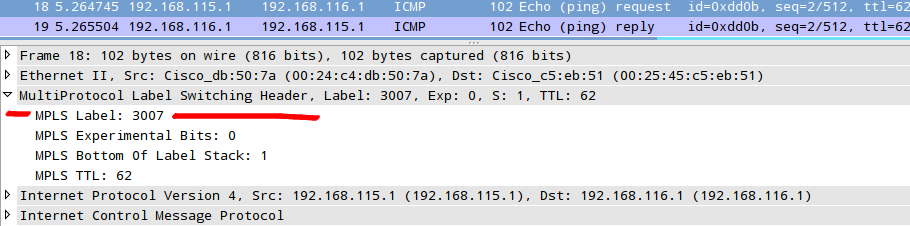
\includegraphics[width=1.0\textwidth]{../e3/ping.png}
\caption{Ping request tagged with label 3007}
\label{fig:mpl1_ping1}
\end{figure}
\begin{figure}
\centering
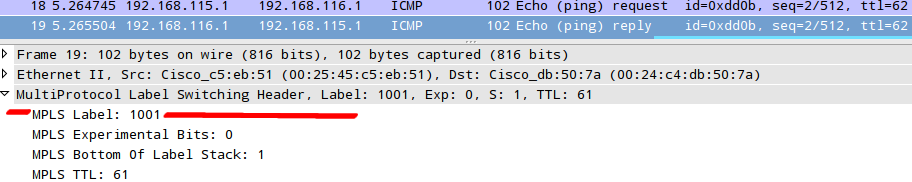
\includegraphics[width=1.0\textwidth]{../e3/pong.png}
\caption{Ping response tagged with label 1001}
\label{fig:mpl1_ping2}
\end{figure}

%===========================================================================
\newpage
\section{VPLS Configuration}
\labelsec{VPLS_config}

This time we modified the basic MPLS test-bed, configured and verified previously, for implementing the Virtual Private LAN Service using MPLS. In fig.\ref{fig:mpls2_topology} is shown the network topology, as always $X=15$ and $Y=16$. 

\begin{figure}
\centering
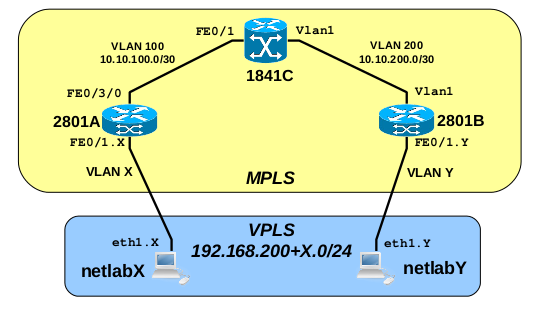
\includegraphics[width=1.0\textwidth]{../e4/topology.png}
\caption{MPLS with Virtual Private Lan Service}
\label{fig:mpls2_topology}
\end{figure}

Configuring VPLS in LER router (Cisco 2801A and 2801B) make MPLS network appear like a chunk of wire, where LER routers behave like network switches.\\
After enabling the $xconnect$ command on both endpoints configuration of LER and LSR change as specified in following dumps.
\begin{verbatim}
(config-if)# xconnect <remote LER router-ID> 1516 encapsulation mpls
\end{verbatim}

\lstset{language=sh, caption=Cisco 2801A (LER) configuration after VPLS set-up, basicstyle=\ttfamily\scriptsize , breaklines=true}
\begin{lstlisting}
 2801A#show xconnect all detail 
Legend: XC ST=Xconnect State, S1=Segment1 State, S2=Segment2 State
UP=Up, DN=Down, AD=Admin Down, IA=Inactive, NH=No Hardware
XC ST  Segment 1                         S1 Segment 2                         S2
------+---------------------------------+--+---------------------------------+--
UP     ac   Fa0/1.15 15(Eth VLAN)        UP mpls 172.30.16.2:1516             UP
            Interworking: none                   Local VC label 1008            
                                                 Remote VC label 2008           
                                                 pw-class:          
                                                             
2801A#show mpls forwarding-table 
Local  Outgoing    Prefix            Outgoing   Next Hop    
tag    tag or VC   or Tunnel Id      interface              
1002   Pop tag     10.10.100.200/32  Fa0/3/0    10.10.100.1  
1003   Pop tag     10.10.200.0/30    Fa0/3/0    10.10.100.1  
1004   3006        172.30.16.2/32    Fa0/3/0    10.10.100.1  
1008               l2ckt(1516)       none       point2point  <==Fwd to tunnel
\end{lstlisting}

According to the VPLS configuration implemented, host in the same VLAN should not be aware of the chunk of MPLS network they cross, in fact a $traceroute$ between 2 host should manifest a single hop.\\

\lstset{language=sh, caption=Traceroute from hosts in the same VLAN, basicstyle=\ttfamily\scriptsize , breaklines=true}

\begin{lstlisting}
$ traceroute 192.168.215.15
traceroute to 192.168.215.15 (192.168.215.15) , 30 hops max , 60 byte packets

1 192.168.215.15 (192.168.215.15) 1.070 ms 1.044 ms 1.039 ms
\end{lstlisting}

\begin{figure}
\centering
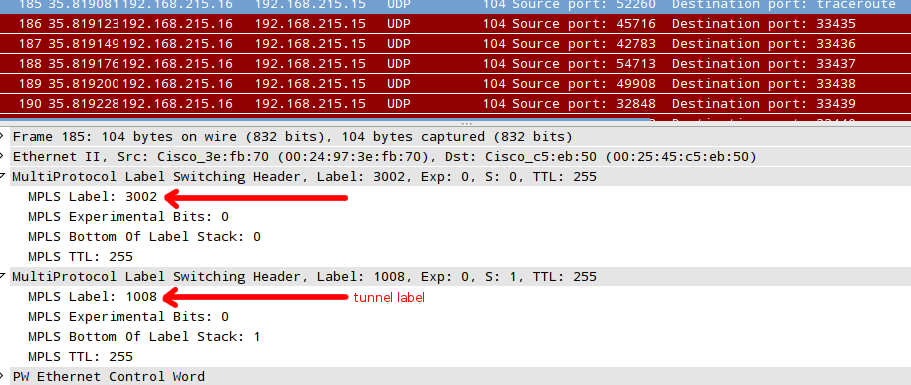
\includegraphics[width=1.0\textwidth]{../e4/traceroute_vpls.png}
\caption{Capture of the traceroute between hosts in the same VLAN, note the stacked MPLS label.}
\label{fig:mpls2_traceroute_vpls}
\end{figure}

%===========================================================================
\newpage
\section{MPLS Traffic-Engineering}
\labelsec{MPLS_te}

In this laboratory session we enable MPLS Traffic Engineering extensions. In fig.\ref{fig:mpls3_topology} is shown the network topology, as always $X=15$ and $Y=16$. 

\begin{figure}
\centering
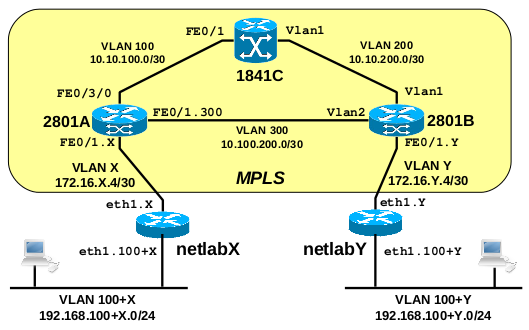
\includegraphics[width=1.0\textwidth]{../e5/topology.png}
\caption{MPLS with TE test-bed}
\label{fig:mpls3_topology}
\end{figure}


Initially - before the configuration of the TE extensions - all interfaces have the same cost, so traffic between VLAN 115 and VLAN116 will NOT pass through Cisco 1841C due to the higher cost of the path.\\

\lstset{language=sh, caption=Traceroute from a host in VLAN115., basicstyle=\ttfamily\scriptsize , breaklines=true}
\begin{lstlisting}
$ traceroute 192.168.116.1
traceroute to 192.168.116.1 (192.168.116.1), 30 hops max, 60 byte packets
 1  192.168.115.2 (192.168.115.2)  0.193 ms  0.175 ms  0.168 ms
 2  172.16.15.6 (172.16.15.6)  1.525 ms  1.822 ms  2.135 ms
 3  10.100.200.2 (10.100.200.2)  1.763 ms  2.018 ms  2.205 ms   <== 2801B
 4  172.16.16.5 (172.16.16.5)  1.038 ms  1.060 ms  1.042 ms
 5  192.168.116.1 (192.168.116.1)  1.055 ms  1.058 ms  1.063 ms
\end{lstlisting}

In order to implement custom traffing engineering policies we had to enable MPLS TE on each MPLS router (LSR/LER), enable RSVP-TE for label distribution with traffic engineering and also enable MPLS-TE within OSPF:
\begin{verbatim}
(config)# mpls traffic-eng tunnels
(config)# interface <interface name>
(config-if)# mpls traffic-eng tunnels
(config-if)# ip rsvp bandwidth <bandwidth in kbps>
(config)# router ospf <processID>
(config-router)# mpls traffic-eng area <area>
(config-router)# mpls traffic-eng router­id <interface name>
\end{verbatim}
And then configure the ingress LER with our custom PATH and create a tunnel interface as entry point for the TE-Path.
\begin{verbatim}
(config)# ip explicit-path identifier <pathID> enable
(cfg-ip-expl-path) # next-address <next-hop-ip>
...
(config)# interface Tunnel <index>
(config-if)# ip unnumbered <routerIDiface>
(config-if)# tunnel destination <routerID>
(config-if)# tunnel mode mpls traffic-eng
(config-if)# tunnel mpls traffic-eng autoroute announce
(config-if)# tunnel mpls traffic-eng bandwidth <bandwidth-kbps>
(config-if)# tunnel mpls traffic-eng path­option 1 explicit identifier <pathID>
\end{verbatim}

In our case we created a TE-Path from 2801A to 2801B through 1841C, in fig.\ref{fig:mpls3_rsvp_path} is reported the RSVP packet which contains path specification.\\
In fig.\ref{fig:mpls3_rsvp_message} is present a following RSVP packet from 1841C to 2801A - entry point of the te path - where is specified the MPLS label that 2801A must use in order to forward traffic into the tunnel.\\
\\
\begin{figure}
\centering
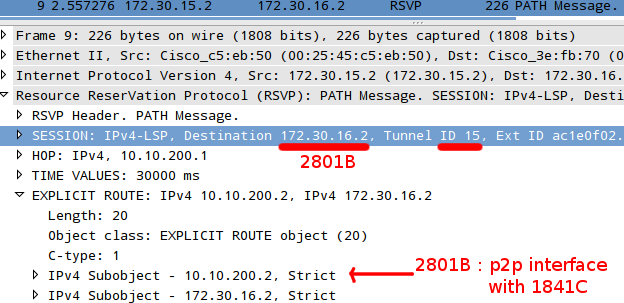
\includegraphics[width=1.0\textwidth]{../e5/rsvp_path.png}
\caption{RSVP Path packet from 2801A to 2801B}
\label{fig:mpls3_rsvp_path}
\end{figure}

\begin{figure}
\centering
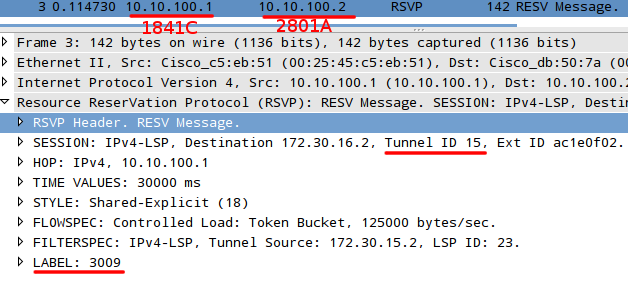
\includegraphics[width=1.0\textwidth]{../e5/rsvp_message.png}
\caption{RSVP packet from 1841C to 2801A with label specification of the tunnel.}
\label{fig:mpls3_rsvp_message}
\end{figure}
\newpage
\lstset{language=sh, caption=2801A Traffic Engineering tunnels., basicstyle=\ttfamily\scriptsize , breaklines=true}
\begin{lstlisting}
2801A#show mpls traffic-eng tunnels 

Name: 2801A_t15                           (Tunnel15) Destination: 172.30.16.2
  Status:
    Admin: up         Oper: up     Path: valid       Signalling: connected

    path option 1, type explicit 1516 (Basis for Setup, path weight 2)

  Config Parameters:
    Bandwidth: 1000     kbps (Global)  Priority: 7  7   Affinity: 0x0/0xFFFF
    Metric Type: TE (default)
    AutoRoute:  enabled   LockDown: disabled  Loadshare: 1000     bw-based
    auto-bw: disabled

  InLabel  :  - 
  OutLabel : FastEthernet0/3/0, 3009					<====
  RSVP Signalling Info:
       Src 172.30.15.2, Dst 172.30.16.2, Tun_Id 15, Tun_Instance 23
    RSVP Path Info:
      My Address: 10.10.100.2   
      Explicit Route: 10.10.100.1 10.10.200.2 172.30.16.2 		<====
      Record Route:  NONE
      Tspec: ave rate=1000 kbits, burst=1000 bytes, peak rate=1000 kbits  <==
    RSVP Resv Info:
      Record Route:  NONE
      Fspec: ave rate=1000 kbits, burst=1000 bytes, peak rate=1000 kbits
  History:
    Tunnel:
      Time since created: 12 minutes, 10 seconds
      Time since path change: 46 seconds
    Current LSP:
      Uptime: 46 seconds
\end{lstlisting}
\newpage
\lstset{language=sh, caption=Forwarding table of 2801A after TE. Tunnel tagging is implicit., basicstyle=\ttfamily\scriptsize , breaklines=true}
\begin{lstlisting}
2801A#show mpls forwarding-table 
Local  Outgoing    Prefix            Bytes tag  Outgoing   Next Hop    
tag    tag or VC   or Tunnel Id      switched   interface              
1000   Untagged[T] 172.16.16.4/30    0          Tu15       point2point  
1001   Untagged    172.30.15.1/32    0          Fa0/1.15   172.16.15.5  
1002   Pop tag     10.10.100.200/32  0          Fa0/3/0    10.10.100.1  
1003   Pop tag     10.10.200.0/30    0          Fa0/3/0    10.10.100.1  
1004   Pop tag [T] 172.30.16.2/32    0          Tu15       point2point  
1005   Untagged    192.168.115.0/24  0          Fa0/1.15   172.16.15.5  
1006   Untagged[T] 172.30.16.1/32    0          Tu15       point2point  <====
1007   Untagged[T] 192.168.116.0/24  0          Tu15       point2point  <====
\end{lstlisting}

Also we can show that LSA type 10 \emph{''opaque``} updates have been propagated through area 0. 
Opaque LSAs contain information which should be flooded by other routers, they are typically used for traffic engineering extensions to OSPF. Extra informations might include link bandwidth. In the following code listing is shown that 2801A has received type 10 LSA.
\\
\lstset{language=sh, caption=2801A OSPF database with type 10 LSA, basicstyle=\ttfamily\scriptsize , breaklines=true}
\begin{lstlisting}
2801A#show ip ospf 15 database 

            OSPF Router with ID (172.30.15.2) (Process ID 15)

		Router Link States (Area 0)
Link ID         ADV Router      Age         Seq#       Checksum Link count
10.10.100.200   10.10.100.200   767         0x80000137 0x00A7D6 4
172.30.15.1     172.30.15.1     180         0x8000000B 0x00BE50 3
172.30.15.2     172.30.15.2     1503        0x80000270 0x00D91A 4
172.30.16.1     172.30.16.1     180         0x8000000A 0x0013F6 3
172.30.16.2     172.30.16.2     1504        0x8000026A 0x009549 5
		Net Link States (Area 0)
Link ID         ADV Router      Age         Seq#       Checksum
10.10.100.2     172.30.15.2     1949        0x8000012D 0x009A02
10.100.200.2    172.30.16.2     1504        0x80000001 0x002549
172.16.15.5     172.30.15.1     180         0x80000002 0x008D6C
172.16.16.5     172.30.16.1     180         0x80000002 0x009164
		Type-10 Opaque Link Area Link States (Area 0)
Link ID         ADV Router      Age         Seq#       Checksum Opaque ID
1.0.0.0         10.10.100.200   1022        0x80000001 0x0083B2 0       
1.0.0.0         172.30.15.2     134         0x80000002 0x009BC3 0       
1.0.0.0         172.30.16.2     135         0x80000001 0x0035A8 0       
1.0.0.1         10.10.100.200   136         0x80000002 0x0069BC 1	<====
\end{lstlisting}

The correct establishment of the traffic engineering path is also verifiable by trace-routing traffic from VLNA115 to VLAN116 where packets are forwarded in the TE tunnel.\\
Traffic from VLAN116 to VLNA115, instead, are forwarded through the shortest path due to the absence of tunnel specification for the opposite direction.

\lstset{language=sh, caption=Traceroute from VLNA115 to VLAN116 after TE, basicstyle=\ttfamily\scriptsize , breaklines=true}
\begin{lstlisting}
traceroute 192.168.116.1
traceroute to 192.168.116.1 (192.168.116.1), 30 hops max, 60 byte packets
 1  192.168.115.2 (192.168.115.2)  0.217 ms  0.196 ms  0.182 ms
 2  172.16.15.6 (172.16.15.6)  1.266 ms  1.750 ms  2.129 ms
 3  10.10.100.1 (10.10.100.1)  1.533 ms  1.662 ms  1.839 ms	<==== 1841C 
 4  10.10.200.2 (10.10.200.2)  1.898 ms  2.201 ms  2.259 ms
 5  172.16.16.5 (172.16.16.5)  1.025 ms  1.026 ms  0.854 ms
 6  192.168.116.1 (192.168.116.1)  0.924 ms  0.932 ms  0.921 ms
\end{lstlisting}

\lstset{language=sh, caption=Traceroute from VLNA116 to VLAN115 after TE, basicstyle=\ttfamily\scriptsize , breaklines=true}
\begin{lstlisting}
traceroute 192.168.115.1
traceroute to 192.168.115.1 (192.168.115.1), 30 hops max, 60 byte packets
 1  192.168.116.2 (192.168.116.2)  0.202 ms  0.186 ms  0.165 ms
 2  172.16.16.6 (172.16.16.6)  1.314 ms  1.715 ms  2.029 ms
 3  10.100.200.1 (10.100.200.1)  1.884 ms  2.122 ms  2.317 ms 	<== to Vlan2
 4  172.16.15.5 (172.16.15.5)  1.260 ms  1.301 ms  1.283 ms
 5  192.168.115.1 (192.168.115.1)  1.278 ms  1.265 ms  1.253 ms
\end{lstlisting}
%===========================================================================
\newpage
\section{Hierarchical Token Bucket}
\labelsec{HTB_ts}

In this laboratory session we enable reused previous MPLS network as transport network and realize a QoS policy through traffic shaping. In fig.\ref{fig:qos_topology} is shown the network topology, as always $X=15$ and $Y=16$. 

\begin{figure}
\centering
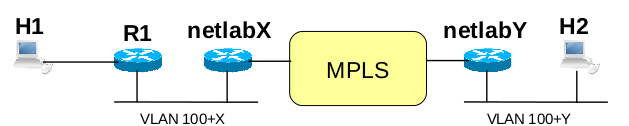
\includegraphics[width=1.0\textwidth]{../e6/topology.png}
\caption{MPLS with TE test-bed}
\label{fig:qos_topology}
\end{figure}

The main goal of this experience was to deploy 3 class of service for VLAN115's outgoing traffic, with different reserved bandwidth:
\begin{itemize}
\item class 1 :  dport 3001, rate 1 Mbps,  label 12\begin{list}{}{} \small \item DSCodePoint: AssureForwarding, class 1, medium drop precedence \end{list}
\item class 2 :  dport 3002, rate 2 Mbps,  label 20 \begin{list}{}{} \small \item DSCodePoint: AssureForwarding, class 2, medium drop precedence \end{list}
\item class 3 :  dport 3010, rate 10 Mbps,  label 36 \begin{list}{}{} \small \item DSCodePoint: AssureForwarding, class 4, medium drop precedence \end{list}
\item class 4 :  best effort
\end{itemize}

In detail we implement a DiffServ architecture, where edge router (R1) classify incoming packets and mark them with proper DS code in IP QoS field, and core router (netlab15) apply appropriate actions based on DS code value.\\


\lstset{language=sh, caption=R1 packet classification using iptables mangle, basicstyle=\ttfamily\scriptsize , breaklines=true}
\begin{lstlisting}
iptables -t mangle -A FORWARD -p tcp --dport 3001 -j DSCP --set-dscp 12
iptables -t mangle -A FORWARD -p tcp --dport 3002 -j DSCP --set-dscp 20
iptables -t mangle -A FORWARD -p tcp --dport 3010 -j DSCP --set-dscp 36

iptables -t mangle -L FORWARD -n
Chain FORWARD (policy ACCEPT)
target     prot opt source       destination         
DSCP       tcp  --  0.0.0.0/0    0.0.0.0/0    tcp dpt:3001 DSCP set 0x0c 
DSCP       tcp  --  0.0.0.0/0    0.0.0.0/0    tcp dpt:3002 DSCP set 0x14 
DSCP       tcp  --  0.0.0.0/0    0.0.0.0/0    tcp dpt:3010 DSCP set 0x24 
\end{lstlisting}

In netlab15 router have been configured the traffic shaper using Hierarchical Token Bucket implementated in $tc$ linux command. But, in order to permit $tc$ to access to packet DSCP values  we had to use iptable parser to read that value and mark the packet in a suitable way for $tc$.

\lstset{language=sh, caption=From DSCP to internal-marking (netlab15), basicstyle=\ttfamily\scriptsize , breaklines=true}
\begin{lstlisting}
iptables -t mangle -A POSTROUTING -o eth1.15 -m dscp --dscp 12 -j MARK --set-mark 12
iptables -t mangle -A POSTROUTING -o eth1.15 -m dscp --dscp 20 -j MARK --set-mark 20
iptables -t mangle -A POSTROUTING -o eth1.15 -m dscp --dscp 36 -j MARK --set-mark 36
\end{lstlisting}

\lstset{language=sh, caption=Configuration of the traffic shaper (netlab15), basicstyle=\ttfamily\scriptsize , breaklines=true}
\begin{lstlisting}
 ---- Set-up Hierarchical Token Bucket ---- 
 
# tc qdisc del dev eth1.15 root
# tc qdisc add dev eth1.15 root handle 1: htb default 0
# tc class add dev eth1.15 parent 1: classid 1:1 htb rate 1mbit
# tc class add dev eth1.15 parent 1: classid 1:2 htb rate 2mbit
# tc class add dev eth1.15 parent 1: classid 1:10 htb rate 10mbit

 ---- Set-up Stochastic Fairness Queueing parameters ---- 
 
# tc qdisc add dev eth1.15 parent 1:1 handle 11: sfq perturb 10
# tc qdisc add dev eth1.15 parent 1:2 handle 21: sfq perturb 10
# tc qdisc add dev eth1.15 parent 1:10 handle 101: sfq perturb 10

 ---- Map packet's internal-mark value to Token Bucket ---- 
 
# tc filter add dev eth1.15 parent 1: protocol ip prio 1 handle 12 fw flowid 1:1
# tc filter add dev eth1.15 parent 1: protocol ip prio 1 handle 20 fw flowid 1:2
# tc filter add dev eth1.15 parent 1: protocol ip prio 1 handle 36 fw flowid 1:10

# tc qdisc show dev eth1.15
qdisc htb 1: root refcnt 2 r2q 10 default 0 direct_packets_stat 43
qdisc sfq 11: parent 1:1 limit 127p quantum 1518b perturb 10sec 
qdisc sfq 21: parent 1:2 limit 127p quantum 1518b perturb 10sec 
qdisc sfq 101: parent 1:10 limit 127p quantum 1518b perturb 10sec 
# tc filter show dev eth1.15
filter parent 1: protocol ip pref 1 fw 
filter parent 1: protocol ip pref 1 fw handle 0xc classid 1:1 
filter parent 1: protocol ip pref 1 fw handle 0x14 classid 1:2 
filter parent 1: protocol ip pref 1 fw handle 0x24 classid 1:10 
\end{lstlisting}

After this set-up we used $iperf$ and $wireshark$ to collect statistics about traffic. The measured average bandwidths are slightly different each other, in fact statistics performed with $ipref$ present a lower bandwidth than the configured one, while $wireshark$ shows higher values.\\
This discrepancy could be derived on a different way in counting transmitted bits, in fact the higher values of $wireshark$ can be explained by considering Ethernet frame and IP header overhead.\\
 
\begin{center}
\begin{tabular}{ l || c | c }
   Class & Bandwidth ($ipref$) & Bandwidth ($wireshark$) \\  
  \hline                        
  1 & 0.92 Mbits/sec &  1.18 Mbits/sec \\
  2 & 1.89 Mbits/sec & 2.31 Mbits/sec \\
  3 & 9.55 Mbits/sec & 11.52 Mbits/sec \\
  4a & 41.2 Mbits/sec & N/A \\
  4b & 38.8 Mbits/sec & N/A \\
  \hline  
\end{tabular}
\end{center}

%===========================================================================
\bibliographystyle{abbrv}
\bibliography{biblio}


\appendix

\section{Collected Data and Logs}
Collected logs and capture files are available at \url{https://github.com/luca-m/ProgRetiLM1213/tree/master/e1} , \url{https://github.com/luca-m/ProgRetiLM1213/tree/master/e2} , \url{https://github.com/luca-m/ProgRetiLM1213/tree/master/e3} , \url{https://github.com/luca-m/ProgRetiLM1213/tree/master/e4} , \url{https://github.com/luca-m/ProgRetiLM1213/tree/master/e5} , \url{https://github.com/luca-m/ProgRetiLM1213/tree/master/e6}.\\
Data and logs has been collectively collected with other group members.

\end{document}












